\chapter{State of Art}
\label{chap:StateofArt}
In this chapter, first section [\ref{sec:HCI}] is dedicated for discussion
related to HCI, its goal and adaptive HCI. In the second section [\ref{sec:ID}],
I have discussed interaction design, its processes, goals, principles and
usability heuristics. In the following sections [\ref{sec:IMA}, \ref{sec:RMA}],
I have discussed interactive mobile application and some related mobile
applications from google play store, which offers some similar feature as like
our proposed ``Smart Cafeteria'' application respectively.

\section{Human Computer Interaction}
\label{sec:HCI}
Human Computer Interaction is a area of research and study which deal with
analysis, design of interactive application by involving its users in
the design process; and focuses on the interaction between Human and computer
application. In some cases, HCI is also known as man-machine interaction (MMI) or
computer-human interaction (CHI). In recent years, there was a great progress in
the field of Mobile human interaction which invloves interaction between users
and mobile applications.

According to \citet{Love:2005:UMH:1076935},  HCI is concerned with looking into
the relationship between human and computer systems and applications that people
use on their everyday life. Since HCI or Mobile Human Interaction is concerned
with investigating the relationship between people and systems or applications,
we are always concerned with understanding the users as well as their various
capabilities and expectations and how these can be taken place into the mobile
system or application design. In the any HCI design process or Interactive
mobile system design, User should be emphasized first and then the other key
aspects are firstly what tasks users want to perform when using the system;
secondly which characteristics of the user could have a significant effect on
their performance with the system; thirdly developing  the system which meet the
users needs and finally the evaluation of the developed system should check if
it meets users' needs as well as satisfying to use and getting users' feedback
which helps to develop updated version of the system. So this includes the
factors such as an understanding of the user and their task what they want to
perform in the system,  the design tools and software packages that are needed
to achieve usability of the system.

\citet{Yang2009} state that the ultimate goal of Human-Computer Interaction
research is exploring how to design the computer or system application to help
people to complete the necessary tasks more safely and efficiently. However the
computer is still a tool and in that case, people and the computer communicate
with each other through the system interface consisting hardware and software. To
achieve that communication effectively and efficiently is called interactive
system design methodology. The main thing is that are those communication really
efficient and effective or enjoyable during usage? All these questions
and answers we will figure out in HCI research work.


\subsection{HCI Goals}
The basic goal of Human-Computer Interaction is to improve interaction between
users and computer  by making applications and computers more usable and
receptive to the user's needs. That means that we want to make the system easy,
safe, effective and enjoyable and to decrease  barrier as much as possible
between human's cognitive model and  user tasks \cite{Sandrahci}. The principle
aim of Human Computer Interaction is to design interactive and safe functional
software system with good usability.

Basically Human Computer Interaction concerns about:
\begin{itemize}
\item \textbf{Process of design interfaces, prototypes and their methodologies:}
HCI concerns about designing the best possible interface, prototype and
development considering user needs and  optimizing the design to achieve desired
functionality in term of learnability ,efficiency of use, effectiveness of use,
enjoyable to use.
\item \textbf{Methods for implementing interfaces and prototype:} HCI also
concerns about methods of software developments, software toolkits and
libraries, efficient algorithms for developing inferface, prototypes and
implementing in real products.
\item \textbf{Methods of evaluating and comparing interfaces and prototypes:}
This is one of the most important part in HCI and interactive product design
which involves user interview, review of application that ensure usability of
application.
\item \textbf{Developing new interfaces, prototypes and interaction techniques:}
This part involves in re-design and evaluating the design of the application.
\end{itemize}

\subsection{Adaptive HCI}
Even the most sophisticated machines will be worthless if user cannot use them.
With time HCI has travelled a long way forward from the start of the concept.
Intelligent and Adaptive HCI is a part of HCI with the goal of research to
improve HCI by using smarter and newer technology. HCI has been influenced a lot
by all the researches of AI technology as AI addresses to topics important for
HCI like adaptability and problem solving.

The main aim of the Intelligent HCI is to enhance the flexibility, usability and
the human-computer interaction. This interaction between men and machine is not
limited to computers only but also with all other machine used in our day to day
life like, television, refrigerator, mobile phones, cars. Nowadays most of the
Intelligent HCIs have the ability to learn from the environment and work
accordingly to reach its goal. Intelligent technologies are used to achieve the
intelligent and adaptive HCI but the goal always remains the same which is to
improve the communication between users and machines. Several techniques are
used to achieve this goal like intelligent input technology, user modeling, user
adaptivity, explanation generation.


An adaptive HCI might be a website using regular GUI for selling various
products. This website would be adaptive -to some extent- if it has the ability
to recognize the user and remembers his searches and purchases and intelligently
search, find, and suggest products on sale that it thinks user might need. Most
of these kind of adaptation are the ones that deal with cognitive and affective
levels of user activity \cite{karray2008human}.

\citet{Lo2006} discussed in his paper that identifying the user's
characteristics is the key for developing adaptive Web-based systems. He also
proposed an adaptive architecture
[Figure-~\ref{AdaptiveApplicationArchitecture}] according to that architecture, 
adaptation decision in an adaptive web-based system depends on user
characteristics which is represented in the user model. An adaptive Web-based
system is helpful to deliver information to users more efficiently and
effectively.
\begin{figure}[h!t]
    \centering
        \fbox{
      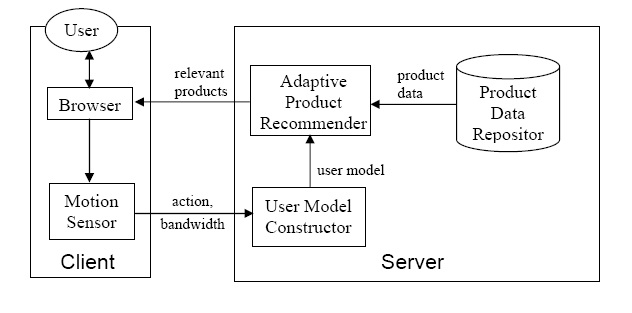
\includegraphics[width=5.5in]{ch2/AdaptiveApplicationArchitecture/adaptive_application_architecture}
      }
  \caption{Adaptive Application Architecture}
  \label{AdaptiveApplicationArchitecture}
\end{figure}

According to his architecture, there are three components in the server: Product
Data Repository, User Model Constructor, and Adaptive Product Recommender. The
Product Data Repository stores the product into database. The User Model
Constructor, together with the observed user browsing behavior, are responsible
for building and updating the temporary user model for incremental learning of
the user's interests. The Adaptive Product Recommender is responsible for
determining the recommendation sequence and the presentation of products in the
user interface based on Product Data Repository and the user model.

\section{Interaction Design}
\label{sec:ID}
A main goal of interaction design is to develop interactive software products
that are usable which means the software should be easy to learn, effective to
use, and should provide an enjoyable experience from the user's perspective
\cite{preece2002interaction}. Designing usable interactive products
requires consideration of the users of software product and the context; means who is
going to use the product and where they are going to be used. Another important
aspect is understands the type of activities performed by users when they
try to interact with the products. The perfectness of different kind of
interfaces and arrangements of input and output factors depends on different type of
activities need to be supported. The aim of interaction design is to provide
redress this concern by bringing usability into the design process. Through
interaction design process, we design interactive products to support people in
their everyday  lives. The main key view of Interactive design is easy,
effortless, and enjoyable.

Interactive system design being a part of Human Computer Interaction is a
multidisciplinary area where various subjects and disciplines such as
Psychology, Computer Science, Sociology, Design contribute its knowledge and
research works supporting on both the machine and the human factors such as
computer user satisfaction. Interactive system design involves several
disciplines and some of them are shown in Figure~\ref{DisciplinesInvolvedID}.
\begin{figure}[h!t]
    \centering
      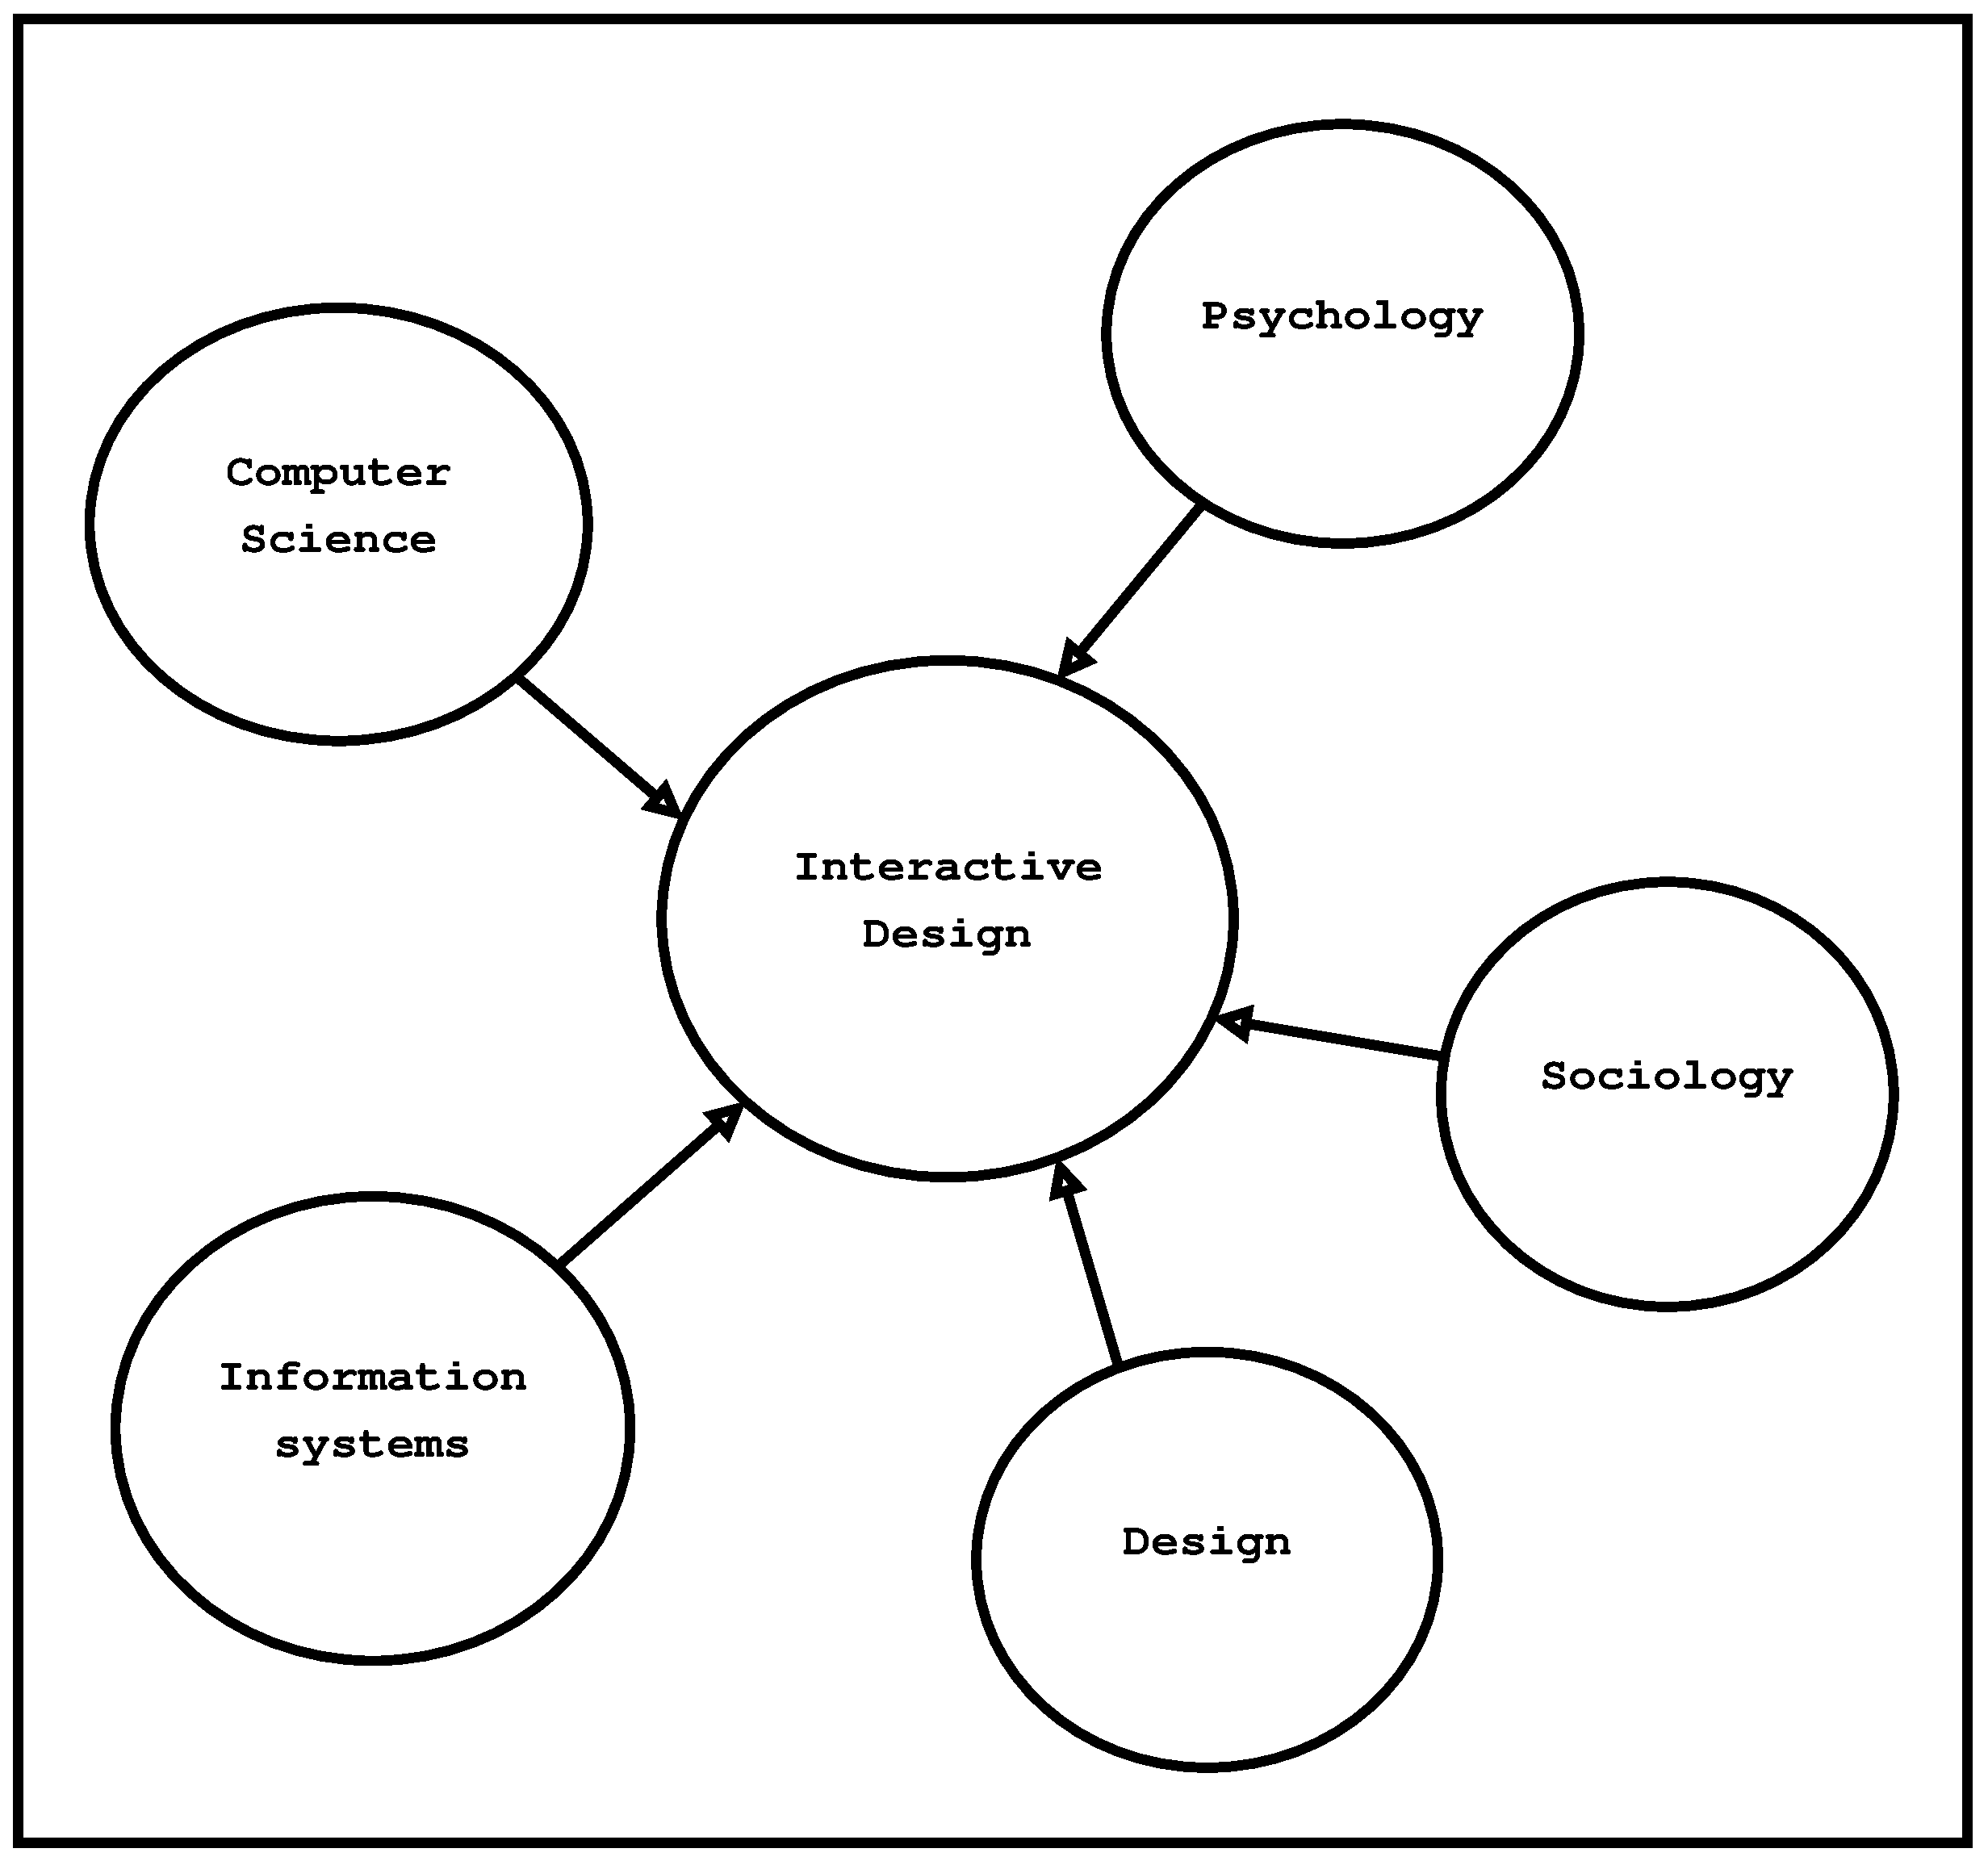
\includegraphics[width=5.5in,height=4in]{ch2/DisciplinesInvolvedID}
  \caption{Disciplines involved in Interactive system design [adapted from \cite{Love:2005:UMH:1076935,preece2002interaction}]}
  \label{DisciplinesInvolvedID}
\end{figure}


\subsection{Interactive Design Process}
According to \citet{Yang2009}, there has not any unique
standard for interactive design in theory, and there's still mainly concept and
model from the software industry. In the field of product design, many new
subjects and situations could happen and the industrial designers need to keep
in practice and study to use the old theory of interaction design principles and
should do more research to sum up  interactive principle and theory which can
suit for target product design and planning. There are three key characteristics
of the interaction design process \cite{preece2002interaction} which should be kept
in mind when we are going to develop any interactive product:
\begin{itemize}
\item Users need to be involved in the development  process.
\item  Specify usability and user experience goals, identify them clearly and
document them properly  at the beginning of the project.
\item  Iteration through the basic four interaction design activities.
\end{itemize}

Fundamentally, the process of interaction design \cite{preece2002interaction} involves four basic
activities:
\begin{enumerate}
\item \textbf{Identifying needs and establishing requirements:} In order to
design some interactive system, we must know about target users and what kind of
services an interactive product could usefully provide.
We should always find out goals and needs of product from the point of view
users. And finally establish a set of requirements which will help to design and
develop product.
\item \textbf{Developing alternative designs that meet those requirements:} This
is the core activity of designing an interactive product which basically suggesting
ideas to meet the requirements. This could  be divided into two sub parts:
conceptual design that means  developing a conceptual model of the product which
describes what the product should do, behave and seems like; and physical design
considers the detail of the product including the colors, sounds, and images of
the product template namely  menu design, icon and interface design.
\item \textbf{Building interactive versions of the designs:} There are sensible
ways for users to evaluate interactive versions of the designs which should be
built, but that does not mean that the final version of the software is required.
There are several techniques to achieve interactive version of product; namely
prototyping, but it does not require a complete software. There are different
prototyping techniques; among them paper-based prototypes are very quick and
cheap for building demo and those are very effective for identifying problems at
the very beginning stages of software design, and through  that  users can get a
real sense of  the product to interact with.
\item \textbf{Evaluating the designs:} Evaluation is the way to determine the
usability and acceptability of product design, which means it is measured
variety of criteria namely the number of errors user make when they are using
it, how attracting it is, how well it matches the requirements, and so on.
Interaction design need  user involvement throughout the development and this
increases quality of the product and confirm final product's quality.
\end{enumerate}
These four steps in interaction design model contains iteration and involves
user in evaluation. From these steps, perhaps some alternative designs could be
generated in some attempts that meet the needs and requirements of the
application. Then interactive design versions of application are developed and
evaluated iteratively. Based on the feedback of the evaluations namely
interviews, users group;  it could return to the step for identifying needs or
refining the previous requirements. In the figure \ref{fig:SimpleLifeCycleID} a
simple lifecycle model of interaction design has been shown\footnote{This image
is adapted from Interaction design: beyond human-computer interaction.}.
\begin{figure}[h!t]
    \centering
      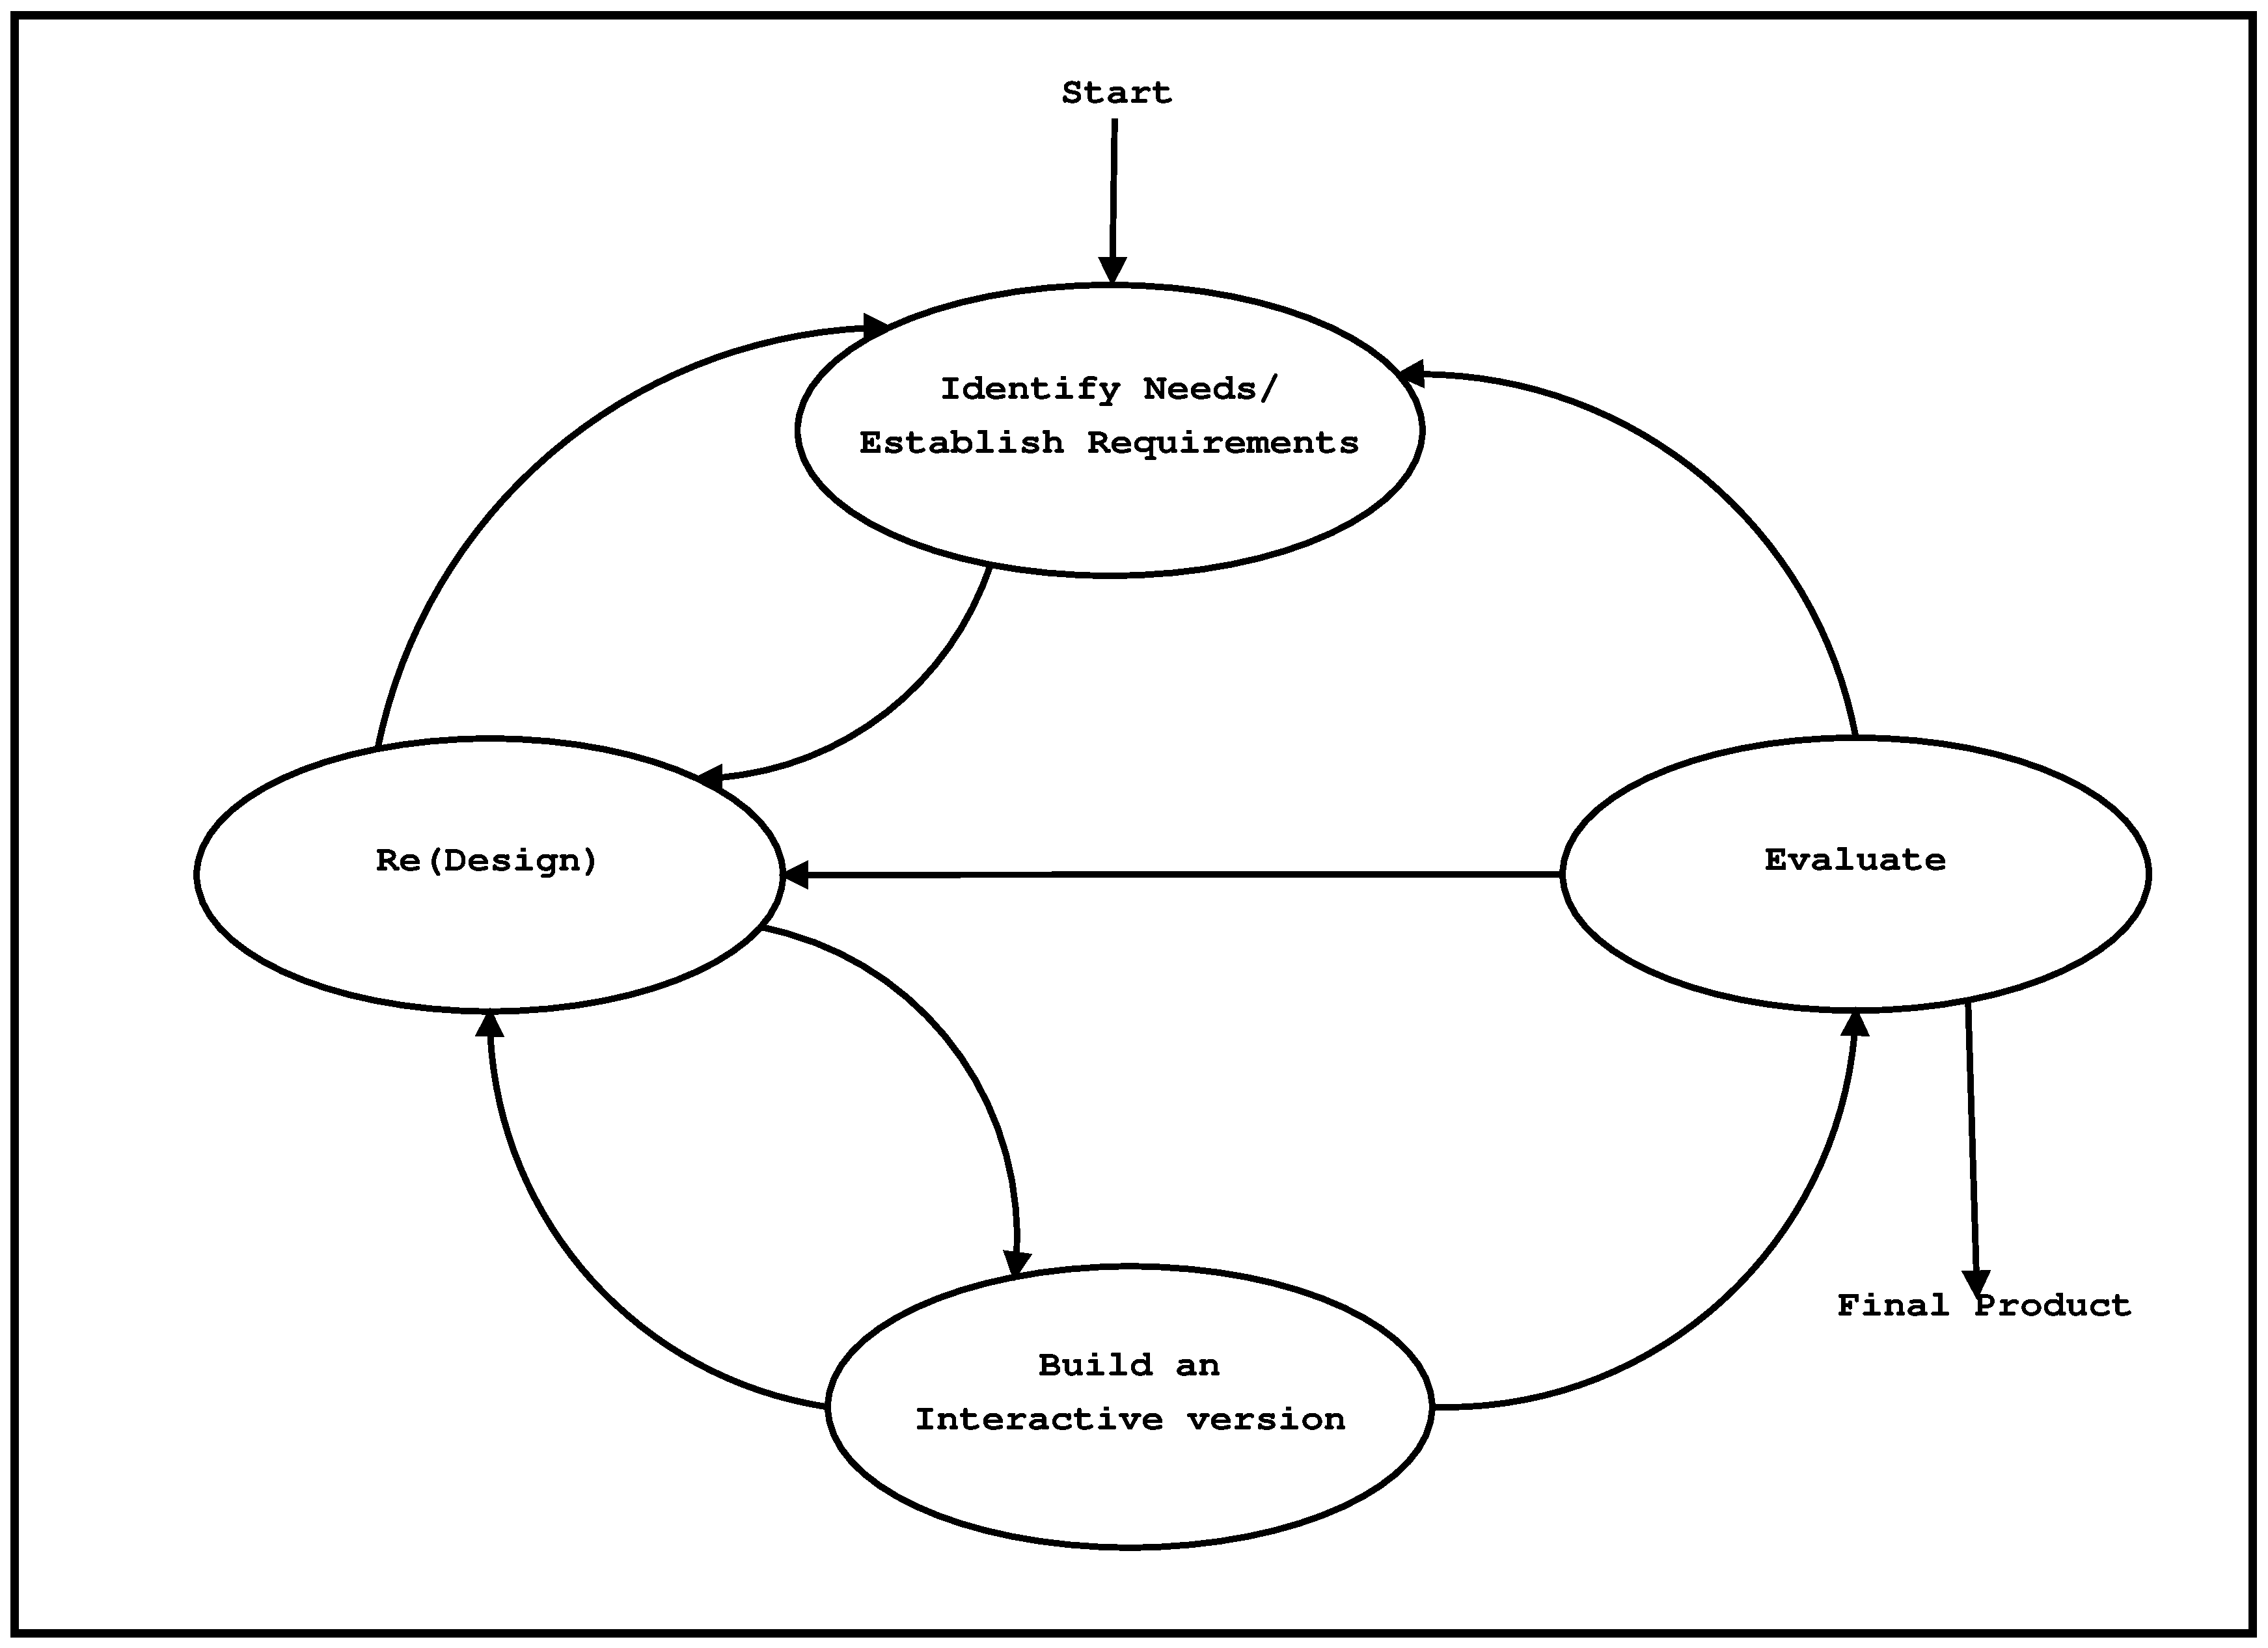
\includegraphics[width=5.5in,height=4in]{ch2/SimpleLifeCycleID}
  \caption{A Simple Life Cycle of Interaction Design Process.}
  \label{fig:SimpleLifeCycleID}
\end{figure}

\subsection{Goals and Principles}
The goals of interactive software design mainly concentrates on usability goals
which ensure that developed applications are easy to learn, efficient to use,
safe to use, effective to use, easy to remember and enjoyable from users'
perspective \cite{preece2002interaction}.
Optimizing alternative connection of people and products are the main objective
of interactive product design. It requires the designers to consider the great
anticipations of the users. Satisfying users' expectation and extending them
to potential needs. Here are the basic principles \cite{Yang2009} of Interactive
product design:

\begin{enumerate}
\item \textbf{Visibility:} In the implementation of application's controls and
functions should follow user perception of the application's operation and the
user's mental model of that application as much as possible. To be compatible
with psychological needs of the users, functions of the product should be
developed in a way so that users can understand and control it properly.

\item  \textbf{Correct and clear feedback:} Somehow  correct and clear feedback
is related with Visibility. Application receives command from different
functions, for execution it should follow a variety of sensory feedback in the
right manner to make access and control of the  system pleasurable, efficient
and canonical.

\item  \textbf{Constraints:} It can be put to practice through physical, logical
and common sense of cultural aspects of interactive product design. Users must
take the correct actions of cross-function to control the enter into the system
forcefully to avoid human errors. To enhance the interaction easy to learn, the
design can be created with safe and reliable use of the environment.

\item  \textbf{Mapping and Matching:} Control of information and
feedback should be able to establish a direct relationship efficiently and
accurately. This is the assurance of user's interactive behavior.

\item \textbf{Consistency:} The psychological vulnerability and memory of user
has a direct impact on the efficiency of the control of the application.  All
the above principles should be followed by the designers in successful
interactive system designs. The designers have to take the psychological feeling
into account and should make the product in a way so that it have a positive
effect in the day-to-day use when they executes the functions.

\end{enumerate}

\subsection{Usability Heuristics}
\label{sec:HeuristicsUsability}
Interactive Design principles incline to be used mainly for developing a new
design, whereas usability principles known as Usability Heuristics are used
mostly as the basis for evaluating prototypes and existing applications. Below
ten usability principles are described which were developed by Nielsen
\cite{Nielsen1990}. Observe that some of them overlap with the interactive
design principles.

\begin{enumerate}
\item \textbf{Visibility of system status:} The system should always inform
users about what is going on in the system and should also provide appropriate
feedback within reasonable time.
\item \textbf{Match between system and the real world:} The system should
provide services using the users' language, rather than system oriented terms
and should follow real world conventions, making information appear in a natural
and logical order.
\item \textbf{User control and freedom:} The system should provide the ways such
as control and freedom to users; if somehow they are stuck somewhere within
system, they could easily escape from that unexpected situation themselves 
using clearly marked emergency exits.
\item \textbf{Consistency and standards:} The system should avoid making users
wonder where different words, actions and situations  mean the same thing and
should follow standard  conventions.
\item \textbf{Help users recognize, diagnose, and recover from errors:} The
system should use plain and easy  language to describe the nature of the problem
and suggest a way to solve it.
\item \textbf{Error prevention:} The system should show relavent error messages
but it is always better to prevent occurrence of errors as much as possible.

\item \textbf{Recognition rather than recall:} The system should minimize the
user's memory load by making objects, actions, and options visible.
\item  \textbf{Flexibility and efficiency of use:} The system should provide
accelerators and flexibility that are invisible to novice users, but allow more
experienced users to carry out tasks more quickly.
\item \textbf{Aesthetic and minimalist design:} The system should avoid using
information which are irrelevant or rarely needed.
\item \textbf{Help and documentation:} The system should provide information
that can be easily searched and help in a set of concrete steps that can easily
be followed.
\end{enumerate}

\section{Interactive Mobile HCI}
\label{sec:IMA}
Mobile Human-Computer Interaction is the relationship (interaction) between
people and their handheld computer systems and the applications which we use in
our everyday life. In a word, mobile applications are interactive products to
support users in their day to day life no matter where they are 
\cite{Love:2005:UMH:1076935}. Since we know from the definition of
interactive system that if a system maintains and follows usability heuristics
and interactive design principles then we can call that system interactive. So
most of the mobile applications are more or less interactive because of their
effectiveness, efficiency, usability and also for their portability.

Mobile applications commonly known as mobile apps are applications developed for
small handheld devices, such as mobile phones, Smartphone's, tablets, PDA and so
on.

Generally mobile application provides the users with similar services which can
be acquired from PCs. Apps are generally small, individual software units with
limited function. They offer limited and confined functionality such as a game,
calculator or even a mobile web browser \cite{JanssenMobileApp}.

The use of mobile application is rapidly growing now a days because of its
portability and usability. In the last couple of year many company and vendor
launched their mobile OS and software platforms to support their PDA. Among
them, Android OS from Google Inc. to support for Android-based devices, iOS from
Apple Inc. to support the iPhone, iPad and iTouch; and Windows Phone from
Microsoft are mostly popular in the market. According to The Telegraph
\cite{Barnett:appslaunched}, in 2011 an average of 701 apps were launched in the
UK version of Apple's App Store every day.  According to The New York Times
\cite{Freierman:appslaunched}, in 2011 an average of 543 apps were released each
day for Android-based devices.

In the Figure \ref{fig:InteractiveMobileApplication} has shown basic interaction
between human and mobile application; and its communication flows.

\begin{figure}[h!t]
    \centering
      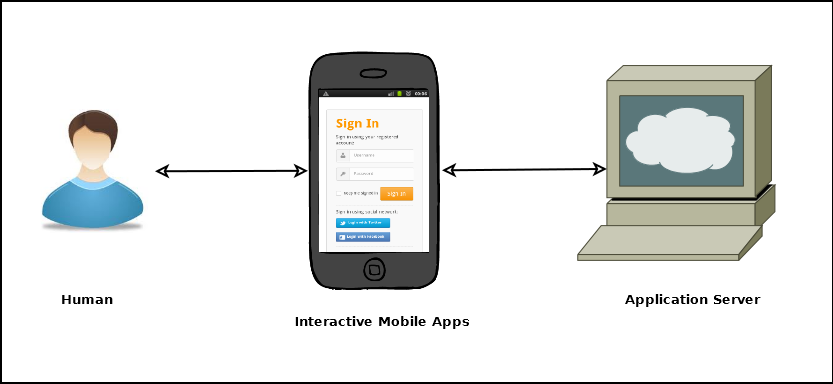
\includegraphics[width=5.5in]{ch2/InteractiveMobileApplication/InteractiveMobileApplication}
  \caption{Interactive Mobile Application}
  \label{fig:InteractiveMobileApplication}
\end{figure}
\newpage
\section{Benchmark Analysis}
\label{sec:RMA}
In order to get the idea about smart cafeteria, I have found some android
applications from Google play store which are similar to my targeted
application. Most of the applications are very light. Although I have not found
all functionalities in single application, so I have chosen couple of
applications to find more requirements and functionalities. In the following
paragraphs I will discuss about some applications which were really helpful for smart
cafeteria.

\begin{enumerate}
\item Calorie Counter-MyFitnessPal\footnote{
\href{https://play.google.com/store/apps/details?id=com.myfitnesspal.android}{Google
Play Store Application-Calorie Counter-MyFitnessPal}.} : This is an Android app
that has largest food database and exercise entry by analyzing those, a fastest
and easiest app to use calorie counter  to diet . It takes input your basic
information such as height, weight, age, gender, your daily activities type and
durations; and your daily food consumptions and exercises; gives you perfect
diet suggestions and generates different reports such as charts of progress over
time and daily nutrition. This application also support social networking such
as friends request and friend invitation.
\begin{figure}[h!t]
\centering
\fbox{
\begin{subfigure}[b]{.33\textwidth}
  \centering
  \fbox{
  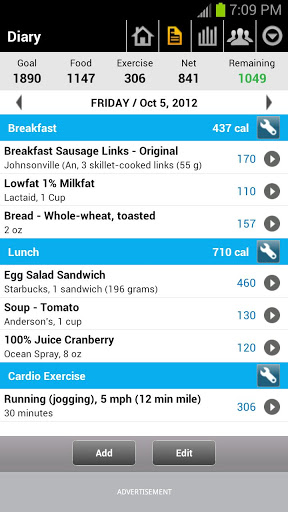
\includegraphics[width=0.9\textwidth]{ch2/RelatedApps/MyFitnessPal/1.jpg}
  }
\end{subfigure}%
\begin{subfigure}[b]{.33\textwidth}
  \centering
  \fbox{
  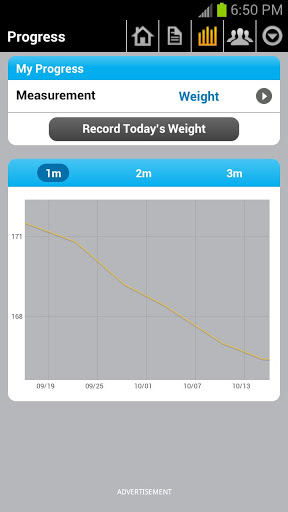
\includegraphics[width=0.9\linewidth]{ch2/RelatedApps/MyFitnessPal/2.jpg}
  }
\end{subfigure}
\begin{subfigure}[b]{.33\textwidth}
  \centering
  \fbox{
  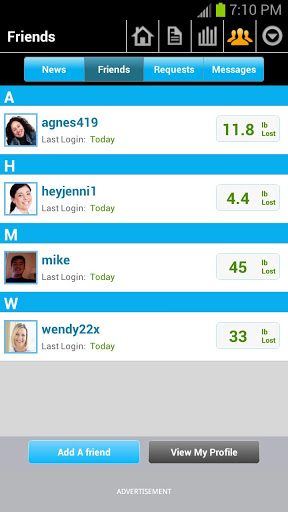
\includegraphics[width=0.9\textwidth]{ch2/RelatedApps/MyFitnessPal/3.jpg}
  }
\end{subfigure}%
}
\caption{Users' Food Diary (left). Users' Progress Report(middle). Users' friends activities (right).}
\label{fig:MyFitnessPal}
\end{figure}
\newpage
\item My Food
Circle\footnote{\href{https://play.google.com/store/apps/details?id=com.multipie.slimcircle}{Google
Play Store Application-My Food Circle}.} : This is a
social~\cite{North51digital} app that helps you instantly share pictures of what
you are eating with your friends. Through this you can connect with people and
friends or you can maintain private food diary.
This app is not only great fun but also can be a big help to stay healthy, lose
weight, eat for fitness, or just enjoy tasty nutritious food. This has also
functionalities like rate one another's meals and share comments, ideas,
encouragement and advice.
\begin{figure}[h!t]
\centering
\fbox{
\begin{subfigure}[b]{.33\textwidth}
  \centering
  \fbox{
  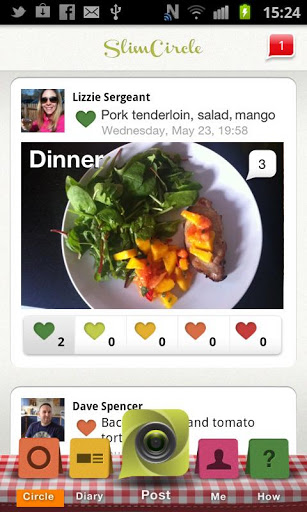
\includegraphics[width=0.9\textwidth]{ch2/RelatedApps/MyFoodCircle/1.jpg}
  }
\end{subfigure}%
\begin{subfigure}[b]{.33\textwidth}
  \centering
  \fbox{
  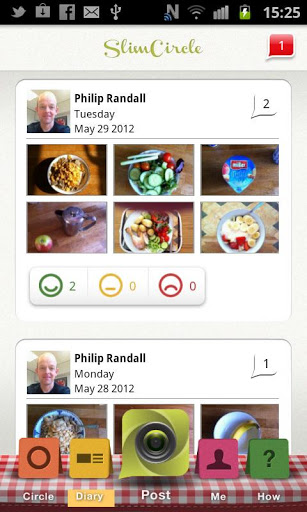
\includegraphics[width=0.9\linewidth]{ch2/RelatedApps/MyFoodCircle/2.jpg}
  }
\end{subfigure}
\begin{subfigure}[b]{.33\textwidth}
  \centering
  \fbox{
  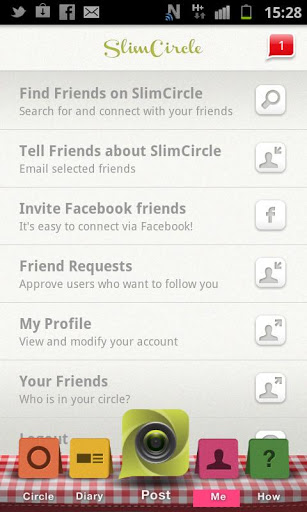
\includegraphics[width=0.9\linewidth]{ch2/RelatedApps/MyFoodCircle/3.jpg}
  }
\end{subfigure}
  }
\caption{Users' wall of My Food Circle (left). User's Food Diary (middle).  Users' functionalities of My Food Circle (right).}
\label{fig:MyFoodCircle}
\end{figure}

\item Restaurant
System\footnote{\href{https://play.google.com/store/apps/details?id=com.aadhk.restaurant}{Google
Play Store Application-Restaurant System}.} :
Restaurant System is a demo android application where customers could order
foods before going to restaurent and also can reserve a table. Waiters also can
use application to check orders from customers' and Chefs receives orders
directly, which are displayed in the monitors placed in the kitchen.

\begin{figure}[h!t]
\centering
\fbox{
\begin{subfigure}[b]{.33\textwidth}
  \centering
  \fbox{
  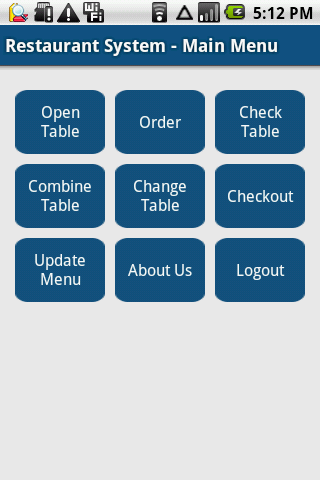
\includegraphics[width=0.9\textwidth]{ch2/RelatedApps/RestaurantSystem/1.png}
  }
\end{subfigure}%
\begin{subfigure}[b]{.33\textwidth}
  \centering
  \fbox{
  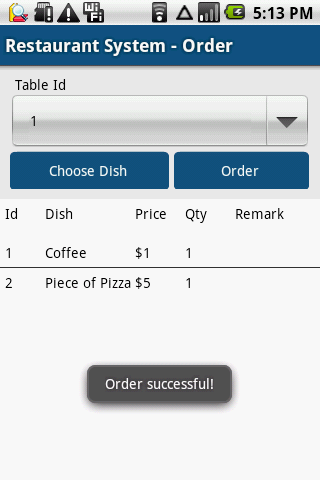
\includegraphics[width=0.9\linewidth]{ch2/RelatedApps/RestaurantSystem/2.png}
  }
\end{subfigure}
\begin{subfigure}[b]{.33\textwidth}
  \centering
  \fbox{
  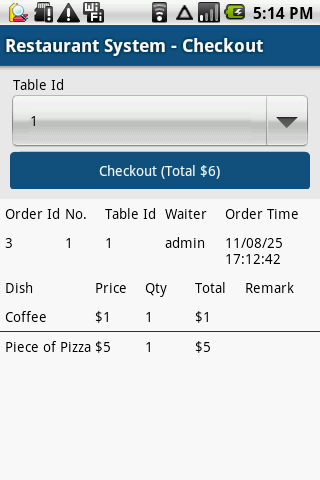
\includegraphics[width=0.9\linewidth]{ch2/RelatedApps/RestaurantSystem/3.png}
  }
\end{subfigure}
}
\caption{Users' Dashboard of Restaurant System(left). Restaurant System Order Dish(middle).  Restaurant System checkout Dish(right).}
\label{fig:RestaurantSystem}
\end{figure}

\end{enumerate}

